% 来源：OEBPS/Text/Section0001_split_008.xhtml#sigil_toc_id_59

\BookChapter{45}
\section[第45章\q 激情的财富]{第45章\\ 激情的财富}

\begin{BookQuote}
只有在激情奋斗时，人才是伟大的。

\hfill ——本杰明·迪斯雷利
\end{BookQuote}

我们一起走了很长的路，是不是？这是一段不可思议的冒险旅程，我非常尊重，非常感激你能够选择和我一起走过这段旅程。

现在，你穿过了那些金钱上的迷思，让它们不再阻挡你通向财务自由之路。你攀爬上财务自由这个财富高山的顶峰，靠的是成功的储蓄和投资，一路坚持，终于实现了你的财务梦想。你学会了新的方式，让你能够顺利而平滑地到达安全又有保障的未来。在那里，你工作只是因为你想要工作，而不是为了赚钱养活自己不得不去工作。

你遇到了一些杰出人物，他们在金融投资上的赚钱能力非凡出众，为人处世品格高尚，努力奉献社会也做得非常好，比如瑞·达利欧、保罗·都铎·琼斯、玛丽·卡拉汉·厄道斯、卡尔·伊坎、戴维·斯文森、约翰·博格、查尔斯·施瓦布，以及其他几十位卓越人士，这些人来帮助指导你走好自己通向财富自由之路。我希望，你阅读本书学到的简单7步投资法，在你的一生中，能够一次又一次地重新阅读、重新回顾、重新学习，让你能够保持对准你的目标，在正确的方向上前进。同时我也会在这部分的末尾，给你提供一个行动清单，帮助你追踪和保持你的前进步伐。将本书所讲作为一种方法来保证你能持续遵守那些基本的原则，以确保你获得财务自由。将来需要的话，重新拿这本书，重新回顾书中的内容，也许就是一种有用的方法，它能提醒你自己，你不是周围环境的创造物，你是自己人生的创造者。记住，知识不是力量，行动才是力量！每一周的每一天，执行都远远胜过知识。

对于我来说，这个旅程是过去几十年学道和传道的顶峰，本书纯粹是我出于爱而心甘情愿的工作成果。本书是我发自内心想要奉献给你的礼物，我希望你能够做得很好，好到你把这份礼物传递给其他人。因为人生最伟大的礼物，就是能够为了某种超越自己生命的东西而活：这份遗产在我们去世之后还会继续增长。

我们快要一起完成这趟旅程了，我希望确认，在我离开你之前提醒过你，我做所有这一切都是为了什么。

我非常荣幸，能够跟各界人士共同合作，包括政治、金融、娱乐、体育等领域的人，也包括宗教和信仰这些精神世界里的人。我曾经在中东开展项目合作，在那里，我把年轻的以色列人和巴勒斯坦人聚到一起，在约旦河西岸组织了一个领导力训练营。一开始，他们彼此表示深切痛恨，但是不到一个星期，他们就成为很好的朋友了。（而且，此后他们在很多和平计划行动上互相支持。）

我从小接受的教导是，没有得到快乐满足的成功是终极的失败。

重要的是，要记住你真正追求的是什么。感觉到快乐、自由、安全和爱，不管你怎么称呼它，就是那种感觉。我们每个人都要找到一条路，通往快乐、满足、意义。路有很多，有些人寻找快乐是通过自然，有些人是通过人际关系。有些人认为，只有身体健康，拥有金钱、学历、优秀的孩子和伟大的商业成就才会让自己感到快乐。但是我们的灵魂深处都知道，真正的财富并不只是你的银行账户存款数字的大小、你拥有的资产规模大小，物质财富并不代表精神财富。

那么，最终的秘诀、富足人生的关键是什么？享受人生，分享人生！但是首先你必须采取行动。俗话说得好，如果你所学的东西只能导向知识，你就学成了傻瓜，如果你所学的东西能够导向行动，你就会变成富人。记住，只有行动才有回报。

所以，在你放下本书之前，复习一下最后的检查核对清单，确认你牢牢记住了通向财务自由之路的这简单的7步，而且你正在路上跟着所学内容前进，正在打造你想要拥有和值得拥有的人生。

检查核对好了，歇口气，放松一下，记住你的目标，所有这些都是为了什么。

\begin{BookQuote}
财富是一种能力，让你完全体验生命。

\hfill ——亨利·戴维·梭罗
\end{BookQuote}

我们都知道有很多种类的财富：情绪财富、关系财富、智力财富、物质财富，它们体现在能量、力量、活力上。当然我们还有精神财富：感觉到我们的生命有更深刻的意义，有超越我们自身的更高层次的召唤。人类容易犯下的最大错误是，当我们专注于某一种形式的财富时，总是以抛弃所有其他形式的财富为代价。

本书从来都不只讨论钱。本书真正讲的是创造一种非凡品质的生活，就是按照你自己的想法来生活。直到现在，我们一直像调整步枪瞄准镜一样重新校准，我们的目标是精通金钱的游戏，实现财务自由，因为这能对你人生的每一件事产生相当大的影响，从心理到健康，再到亲密关系。但是非常重要的是，你要记住，如果你不能精通亲密关系的游戏、快乐满足的游戏、身体健康的游戏，你就根本不可能过上非凡品质的生活。

成为坟墓里面最富有的人，并不是一个好的人生目标。

我永远不会忘记带我的孩子去看太阳马戏团演出的场景。太阳马戏团来到我的老家加利福尼亚州德尔玛镇演出，那是近30年前的事了。我们很幸运，能够买到贵宾票，坐在第一排，紧挨着舞台，几乎一伸手就能碰到台上的演员。

演出马上就要开始了，我注意到身边还空着三个第一排正中间的好座位。我想：“这三个人花大价钱买了这么好的座位，却错过了这么精彩的演出，真是可惜。”但是过了一两分钟，有个体形巨大的人，拄着拐杖，两个人搀扶着他，从楼梯上走了下来，他的体重至少有400斤，往下一坐，一个人就占了三个人的座位。他只是走了几步来到前排，就气喘吁吁，浑身出汗。哎，我真为这个人感到难过，也为我的女儿感到难过，因为他那肥胖的身体，从第三个座位里面挤出来，挤向我女儿的身体！我听到后面有人在小声嘀咕，说他是加拿大首富。我仔细一看，他确实是加拿大最有钱的大富翁。但是在那一刻，我禁不住想，他肯定活得很痛苦，都是因为他把太多的注意力放在赚钱上了，忽略了个人健康，有了巨大的金钱财富，却失去身体健康这种身体上的财富。他实际上正在自杀！由于他不能掌控生活中财富之外的其他方面，所以他不能享受他所拥有的东西，甚至舞台上简单而精彩的一场奇妙马戏表演，他也无法正常观看。

\begin{BookQuote}
我们的内心感受到自身的宝藏，只有在那些时刻我们才可以说我们是活着的。

\hfill ——桑顿·怀尔德
\end{BookQuote}

如果你的生活没有平衡，巨大的成就又有什么意义？如果你从来没有时间庆祝和欣赏你拥有的生活，赢得比赛又有什么意义？一个富有的人经常生气，经常不快乐，还有什么比这更糟的事情？真的没有任何借口，但是我看到这种现象经常发生。这是一种极端不平衡的生活造成的结果，一个人想得到的太多，却没有对自己已经得到的东西有足够多的欣赏。对我们已经拥有的东西没有感恩和欣赏，我们就永远无法体验到真正的满足。正如约翰·邓普顿爵士所说的：“即使你有10亿美元，但是你并不感恩，你就永远是个穷人。即使你只有一点儿钱，但是你对你拥有的这一切充满感恩，那你实际上非常富有。”

如何培养感恩的心？一开始要看清楚控制你大脑和情绪的力量是什么。

我们的决策最终控制着我们的生活品质。这么多年来，我帮助许多人改变了自己的人生，我发现有三个关键的决策是我们生命中每时每刻都在做的。如果我们无意识地做出这三个决策，我们最终拥有的人生就会像大多数人一样身体胖得走形，激情不再，亲密关系变得无聊或者太过舒适，更别提财务紧张了。

但是如果你做出这些决策是有意识的，你就能在一瞬间改变你的生活！这三个决定你生活品质的决策是什么？

\subsection{人生三大关键决策之一：你关注什么？}

生命的每一个时刻，同时会有几百万件事情发生，我们都可以关注。我们关注的事情可以是现在的事物，也可以是未来我们想创造出来的，或者过去的事物。我们可以引导我们的专注力去解决一个巨大的挑战，或者欣赏此刻拥有的美好，或者因为过去那种令人失望的经历而为自己感到遗憾。如果我们没有有意识地引导我们的专注力，我们所处的环境就会不断地提出要求，吸引我们的注意。

有上千亿的资金花在广告上，想得到我们最宝贵的商品——关注。电视新闻为了得到你的关注，会告诉你最可怕的故事：“你的孩子喝果汁会死！快看11点新闻报道！”或者是其他荒谬可笑的说法。为什么？就像它们在媒体上说的“有流血就有高收视率”。如果这还不够，我们生活在一个社交媒体的世界，你口袋里的手机不断地嗡嗡作响，不停地在呼唤你：快看手机。注意，关键是你的注意力在哪里，你的能量就流向哪里，你的关注模式会塑造你的整个人生。

关注模式有很多，我们来看一看其中的两种，它们能够马上改变你感觉到的快乐、幸福、懊恼、愤怒、压力、满足水平。

第一个问题是，你倾向于更多关注的是你有了什么，还是你的人生少了什么。我可以肯定，你会想这就像一个硬币的两面，但是你要好好看一看你的习惯性想法，你倾向于把你大部分时间花费在什么上面。你更关注得到的东西，还是更关注没有得到的东西？

尽管我们之中那些处于极度困难的人，一生中也有很多东西值得好好欣赏。如果你正在财务上挣扎，也许你应该这样想，即使你每年收入只有3.4万美元，在美国只能算是中低水平，但是其实从全世界来看你也属于工资最高的前1/\%，因为全世界所有人口的平均年收入只有1480美元，你的收入水平比全世界平均收入水平高出25倍以上，这样一想是不是心里好受多了？事实上，这个世界上接近一半人，总数超过30亿人，每天只能依靠不到2.5美元的收入维持生活，也就是说，年收入只是略高于900美元。在星巴克喝一杯咖啡平均花费3.25美元。如果你能付得起，那么你购买一杯星巴克咖啡的钱，就超过这个地球上一半人一天必需的生活开支。

这样你能把事情看得更加清楚明白了，是不是？如果你想占领华尔街，因为你憎恨那些收入属于前1\%的有钱人，你也许会停下来想一想，照你这样想，全世界其余99\%的人也想占有你那“糟糕”的生活！

\begin{figure}[htbp]
\centering
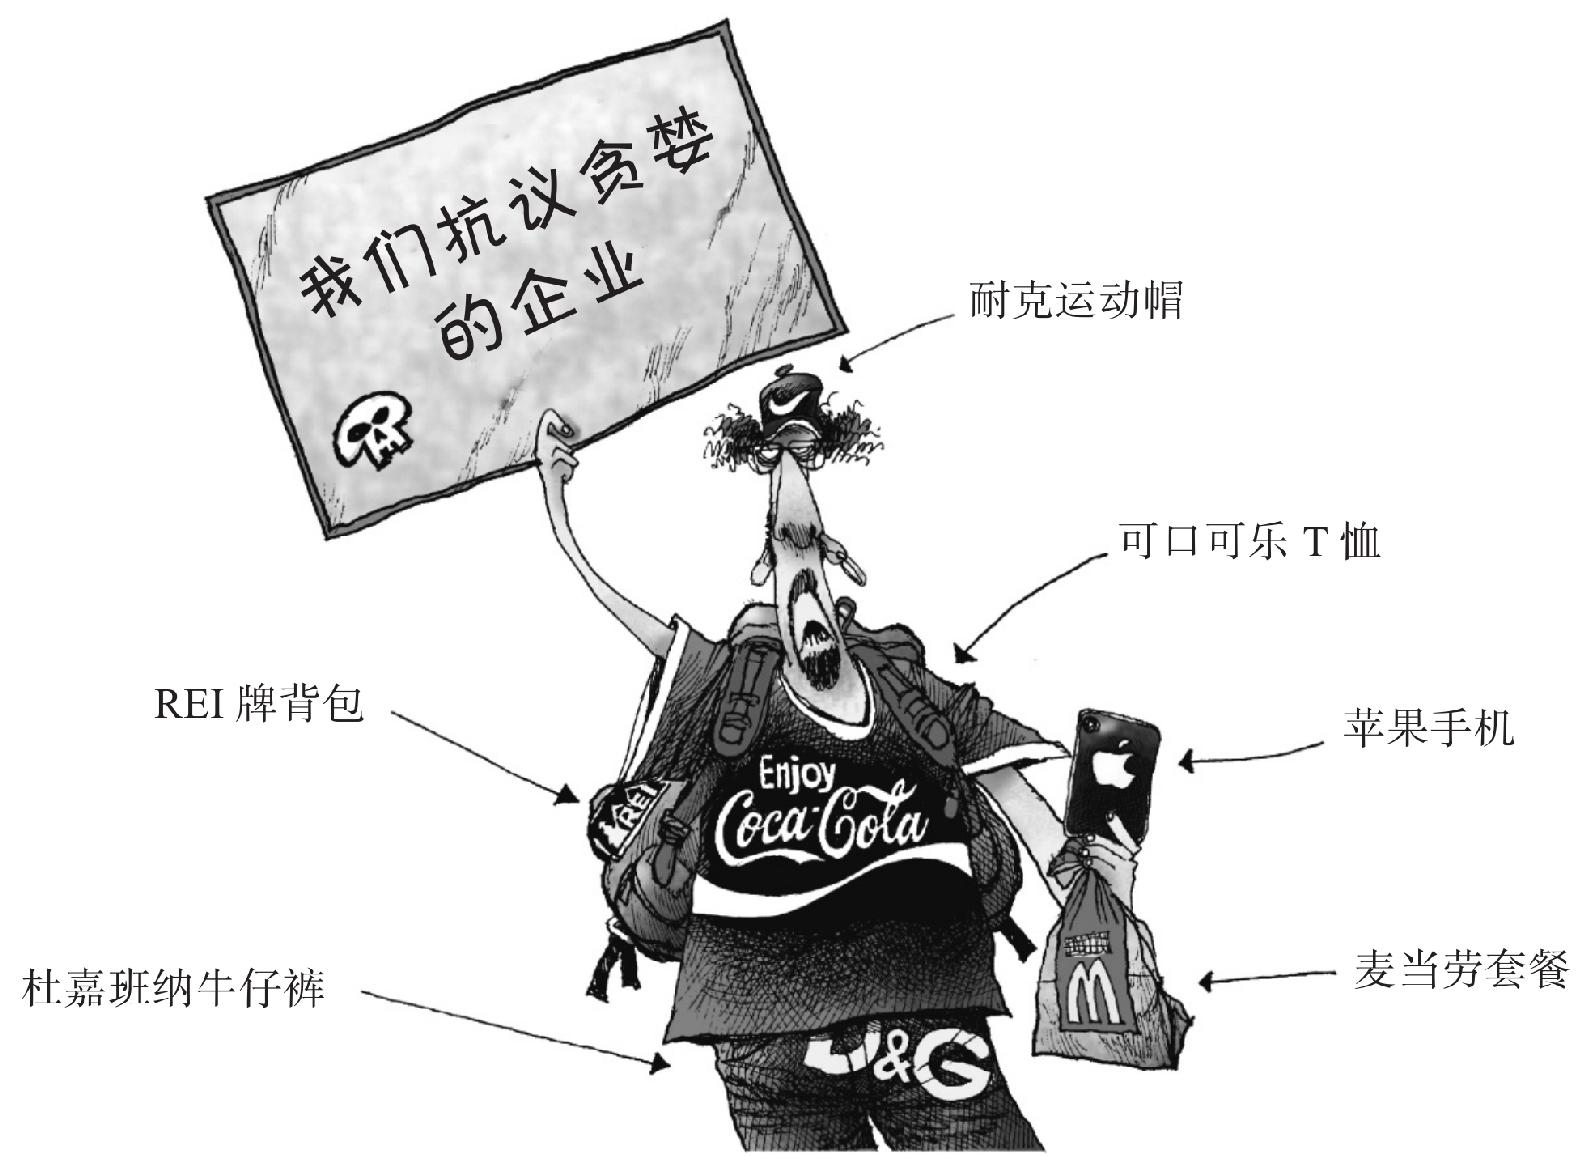
\includegraphics[width=0.78\linewidth,keepaspectratio]{image/45-1.jpg}
\caption{}\label{fig:45-1}
\end{figure}

但是非常严肃地说，与其关注我们并不拥有的东西，或者抱怨那些比我们更有钱的人，也许我们更应该知道，我们的生活已经有很多东西值得我们感恩了，而这些东西都与钱无关。好多地方值得感恩：我们有健康的身体、朋友、机会、头脑，我们能在路上开车前行却不用自己修这些路，可以读书却不用自己花费好几年来写这些书，可以上网却不用我们自己去创造如此庞大的互联网。

你倾向于把专注力放在什么地方，是关注你拥有的东西，还是关注你失去的东西？

欣赏你已经拥有的东西，这种模式可以创造出一种新的心理健康水平和财富水平。我猜想，既然你正在读本书，那么你应该是一个注意到你拥有什么的人。但是真正的问题是：你是否拿出时间，从你的身体深处、内心深处、灵魂深处，深深地感到非常感恩？这才是你能够找到快乐和馈赠的地方。只是知识上的欣赏，或者再多得1美元、多赚1000万美元，都不能给你带来真正的快乐。

我们来看一看第二个会影响到你生活品质的关注模式：你倾向于关注你能控制的东西，还是你不能控制的东西？我知道，这个问题的答案是依具体情况而定的，你会在不同的时刻有不同的回答，但是我问你的是从总体来看，你更倾向于更多地关注你能控制的东西，还是你不能控制的东西。一定要诚实地回答。

如果你关注的是你不能控制的东西，毫无疑问你在生活中会压力更大。你可以管理你生活中的很多方面，但是你不能控制市场，控制那些你关心的人的健康，你也不能控制你孩子的态度，任何一个人和2\textasciitilde{}16岁的孩子一起生活过的人，都明白这一点。

你可以影响很多事情，但是你不能控制这些事情。我们越是感觉失去控制，越会感觉很受挫。事实上要衡量自尊，可以用我们的两种对比来衡量，对我们自己生活中的事件，我们感觉是我们控制这些事件，还是这些事件在控制我们？

现在，你一开始关注某件事情，你的大脑就要做出第二个决策……

\subsection{人生三大关键决策之二：这有什么意义？}

这有什么意义？最终，我们对人生的感受，和我们生活的事件没有任何关系，和我们的财务状况没有任何关系，和发生或者没有发生到我们身上的事情也没有任何关系。控制我们生活品质的，是我们赋予这些东西的意义。大多数时间我没有意识到，这些快速的关于有什么意义的决策，会对我们的人生产生什么影响，因为这些决策通常是我们在无意识状态下做出的。

某件事情的发生一下子打乱了你的生活，例如出车祸、健康出问题、失去工作等，你会倾向于认为这是个结束，还是个开始？如果有人和你作对，他是在“侮辱”你，“教导”你，还是真的“关心”你？这种“非常犀利”的问题意味着，上天是在惩罚你、折磨你，还是有可能这是上天赐给你的礼物？你给你的人生什么意义，你的人生就有什么意义。因为每种意义后面都是一种独特的感觉或者情绪，我们生活的情绪是什么样的，我们生活的品质就是什么样的。

意义并不只影响我们感觉的方式，还会影响我们的亲密关系，我们之间的互动。有些人认为，人际关系的前10年只是开始，过了10年才开始互相了解，这真的令人激动。这是个可以更加深入地了解对方的机会。有些人可能只用10天就建立了亲密关系，而他们一发生争吵就会觉得他们的关系断了。

如果你觉得，这是一段亲密关系的开始，你的行为表现会不会跟你感觉这是一段亲密关系的结束一模一样？感觉上的轻微改变，意义上的轻微改变，就可以在瞬间改变你的整个生活。一段亲密关系刚开始的时候，如果你全心全意地爱对方，全身心都受到对方的吸引，那你会为对方做些什么？答案是：什么事都行！如果对方让你倒垃圾，你会又蹦又跳地说：“只要能让你高兴，亲爱的，我什么都愿意做！”但是过了7天，过了7年，过了17年，有人就会说：“我是你的清洁工吗？”他们会开始困惑，他们生命中这段激情发生了什么问题。我经常跟那些出现感情问题的夫妻分享，如果你能像你们的亲密关系开始时一样做事，那么你们两个人的亲密关系就永远不会走向终结！关键是因为在亲密关系开始的时候，你是一个给予者，而不是一个斤斤计较自己付出了多少又得到了多少的人。你不会不停地掂量给予对方更多有没有意义。你关注的只是让那个人高兴和让那个人开心，只要对方快乐，就会让你感觉你的人生充满快乐。

我们来看看前两个决策：专注和意义，二者经常糅合在一起，创造出现代社会最大的痛苦——抑郁症。我敢肯定你会觉得很奇怪，怎么可能有那么多“富有”又很有名的人患抑郁症？你渴望的每一种资源他们都有。那些名人受到几百万名粉丝的热爱，有几千万美元甚至几亿美元的财富，怎么可能会结束自己的生命？我们一次又一次地看到这种事情发生，其中很多人都特别聪明、有才华，从商人到娱乐明星，再到喜剧演员，都有。这怎么可能？现在有这么多现代治疗方法和药物！

在我组织的大型讲座上，我总是问：“你们中有多少人知道，有人在用抗抑郁药，而且用药之后还是抑郁？”在全世界很多地方，5000\textasciitilde{}10000人的讲座现场，我总是看到现场举起手的人占到85\%\textasciitilde{}90\%。这怎么可能？毕竟，你给了他们药，吃了药应该会让他们感觉好多了呀？

这些抗忧郁药，上面都会写着一句警告：可能会有产生自杀想法的不良反应。但是也许真正的挑战是，不管你给自己吃多少药，如果你的关注点保持在你的人生中自己不能控制或者失去的东西，那么你总是感觉自己处于绝望之中。如果你给这些事件赋予的意义是“人生不值得活下去”，你就等于是喝了能产生绝望情绪的鸡尾酒，没有什么抗抑郁药能持续克服这种情绪。

但是我可以告诉你，毋庸置疑，同一个人，如果找到一种新的人生意义，即让自己活下去的理由，或者相信自己的人生是有意义的信念，那么他的内心就会变得非常强大，任何事情发生在他身上都不能击垮他。如果能随时关注谁需要你、谁爱着你、你还想给予这个世界什么，那么任何人都能改变。你会问：你怎么知道？因为在这38年里，我和很多人一起合作，共同努力，帮助他们走出人生困境。在这好几千人里，没有一个人自杀！祈求上天，保佑我好运，希望我永远不会碰到学员自杀这种事，尽管这种事谁都无法保证。但是如果你能让人们转移他们习惯性的关注点和意义，那么这个人的人生就会变得无限大。

改变关注点，改变意义，能在几分钟内就改变你的生理反应。学会掌握这一点，你会变成一个情绪游戏的改变者。除此之外，你怎么解释，伟大的临床医疗专家和思想家维克多·弗兰克尔和很多人在奥斯威辛集中营那些恐怖的日子里展示出的力量与美好？即使是在极端的痛苦之中，他们也找到了人生的意义。这是更高、更深层次的人生意义，它不但让他们自己活下去，而且将来还能拯救很多人的生命，他们靠的就是相信“这种事再也不会发生了”。我们都能找到意义，即使是在我们的痛苦中。也许，我们找到意义了，我们还是会感觉痛苦，但是那种受苦的感觉消失了。

所以要获得控制，一定要记住：意义就等于情绪，情绪就等于生命。有意识地做明智的选择。在任何事物上找到能赋予你力量的意义。让你感觉最深刻的财富，今天就是你的了。

\subsection{人生三大关键决策之三：我要做什么？}

一旦我们在大脑中创造出一种意义，这个意义就会创造出一种情绪，从而带来一种状态，我们会在这种状态中做出第三个决策：我要去做什么？我们采取的行动，在很大程度上是由我们所处的情绪状态塑造的。如果我们感到生气，这个时候我们的行为就会明显不同于我们感觉好玩的时候，也明显不同于我们感觉狂怒的时候。

如果你想塑造你的行为，最快的办法就是改变你的注意力所在，改变你赋予某件东西的意义，让你自己有更大的自主权。即使是两个人都处在生气发怒的状态，行为也会有很大区别。有些人生气发怒时会向后退，而有些人一生气发怒就会往前猛冲。不同的人表达怒气的方式也不同：有些人很安静；有些人较大声；有些人很强烈；有些人会压抑自己的愤怒，只是为了找一个消极对抗的机会重新占据上风，甚至实施报复；有些人发泄他们愤怒的办法是去健身房，在激烈的健身运动中把情绪发泄出去。

那么这些行为方式是从哪里来的？我们往往是模仿生活中那些我们尊敬、喜欢、热爱的人的行为方式。对那些让我们感到懊恼、让我们生气的人，我们经常排斥他们的行为方式，但是我们常常发现，我们也落得跟他们一样，采取同一种行为方式，这是因为我们年轻的时候一次又一次地亲眼看到这些行为方式，我们非常不喜欢这些行为方式，结果越痛恨印象越深，而且次数多了，我们反而无意识学得最像。

一个非常有效的应对办法是，要变得有意识地觉察，当你懊恼、愤怒、悲伤、感觉孤单的时候，你的行为方式是什么。因为如果你意识不到，就根本没法改变。除此之外，既然你已经意识到了这三种人生关键决策的力量，你也许就会开始寻找自己的人生榜样，你想过的生活，你的榜样已经过上了。我敢向你保证，那些拥有充满激情的亲密关系的夫妻，相比于那些不断吵架甚至打架的夫妻，关注的事情肯定完全不同，对亲密关系中出现的困难也会赋予完全不同的意义。这并不是高深的科学。如果你开始意识到人们如何做出这三大决策有很大的不同，你就找到了一条路，能帮助你创造出永久性的积极改变，在你生活的任何一个领域都行。

\begin{BookQuote}
18岁的时候，我下定决心，我的人生从此再也不会有糟糕的一天。我跳入深不见底的感恩之海中，我永远不会离开。

\hfill ——帕奇·亚当博士
\end{BookQuote}

你能如何运用这三大关键决策来提升你的生活品质？结果表明我们关注什么，我们就容易生活在什么样的情绪状态里，我们做什么都是可以训练出来并养成习惯的，或者都是可以事先安排好的。毕竟你不希望那种积极的情绪只是一闪而过，而是想要训练自己生活在那种积极的情绪之中。这就像一个运动员锻炼某一块肌肉。你必须训练自己，才能得到你想要的那些非凡品质的满足、享受、快乐、成就，在你的个人生活、职业、感情三个生活领域中都是如此。你必须训练自己专注、感觉，找到最能够赋予你能量的意义。

这种实践操作根植于心理学上的一个概念“启动效应”，它的意思是，词语、想法、感觉体验歪曲了我们对这个世界的感觉，进而影响我们的情绪、动机、行动。

如果你发现，你的想法其实只是受到环境的触发，或者是在某些情况下受到懂得激发力量的人有意识地操纵才有的力量，那么你会怎么样？我来给你举个例子。

两个心理学家搞了一项研究，他们让一个陌生人递给实验参与者一杯咖啡，不是一杯热咖啡，就是一杯冰咖啡。接着他们让实验参与者读一篇文章，里面描述了一个假设出来的人物，然后让这些实验参与者描述这个人物的性格。结果令人震惊！那些拿到一杯热咖啡的人描述这个人物的性格是“热情的”“慷慨的”，而那些拿到一杯冰咖啡的人会描述这个人物的性格是“冷淡的”“自私的”。

在华盛顿大学做的另外一项研究中，对有亚洲血统的女士进行一场数学测验。测验之前，他们让这些女士填一个简单的问卷。如果问卷让这些有亚洲血统的女士写上自己的种族，那么她们的数学测验成绩会提高20\%。但是若让这些有亚洲血统的女士填上性别，就是写下来她们是女性这么一个简单的动作，就会明显地降低她们的数学测验分数。这就是文化方面的词语引发启动效应产生的巨大影响。这影响到我们的潜意识模式，缩小或者放大了我们的真实潜力。

我们可以用这种现象来开发一个简单的每日10分钟练习，启动我们的头脑和心灵来感恩，这种感恩的情绪能够消灭恐惧和愤怒。记住，如果你的情绪是感恩的，那么它就不会同时是愤怒的。你的情绪不可能既是恐惧的同时又是感恩的。这是绝对不可能的！

我每天早上至少要做10分钟的感恩练习。我停下来，闭上眼，用3分钟左右想想，我要感恩什么：我脸上的风，我生活中的爱，我得到的机会和福分。我并不只是关注大事，我不仅注意而且深深地感觉到，我非常感激这些能让人生富足的小事情。接下来的3分钟左右，我会祈求上天赐予健康和福气给那些我爱、我了解、我三生有幸接触到的人：我的家人、我的朋友、我的客户和我今天可能会遇到的陌生人。传递爱、祝福、感恩，祝愿所有的人都能富裕安康。这听起来可能有些老掉牙，但是生命的循环就是这样的。

我把余下来的3分钟左右的时间花在我称为“三生万物”的事情上面，即我想成就的三件事。我想象着，这三件事情完成后的情形，感受高兴、庆祝、感恩的感觉。启动效应是你送给自己的一份重要礼物，如果你连续这样做上10天，你就会上瘾，你会欲罢不能。

这个简单的练习很重要，因为很多人说他们心里是感恩的，但是他们并没有花时间去真心感恩。在生活中，很容易忘记我们已经拥有的那些美好和幸福！如果我们不能有意识地每天做些事情，把正确的种子种在我们的头脑里，那些“生命的野草”，即懊恼、愤怒、压力、孤单，就会悄悄地混进你的头脑中。你并没有故意播种野草，它们却会自动生长出来，我的第一个人生导师吉姆·罗恩教给我一个简单的原则：每一天都要站在你的心灵门口当好看门的保安，你自己要决定什么样的想法和信念可以进入你的生命。这些东西将会塑造的情绪感觉，决定你感觉到的是富有还是贫穷，是上天的诅咒还是上天的赐福。

最终，我们若想真正地活得快乐，我们就必须走出自己的狭小天地。

人类的大脑是一个神奇的东西，这是一个生存机制，所以大脑很容易关注哪些东西错了、哪些东西要避开、哪些东西应该小心。你也许已经进化了，但是你的大脑还是那个有200万年历史的结构，如果你想得到的是满足和快乐，这并不是大脑最优先的选择。你必须来控制你的大脑。要做到这一点，最快的办法，除了启动效应之外，就要迈入六大人类基本需要的最高层次需要，就是那两个让人类得以满足的精神需要——成长和奉献。

我相信我们都有成长的渴望，核心原因是我们这样做的时候就有东西去给予。这正是生命最有深刻意义的地方。“得到”也许会让你感觉良好那么一小会儿，但是得到什么东西也比不上给予的终极快乐：你知道，某个能深深地触动你的东西，是超越了你自己的存在。

\begin{BookQuote}
每个人都能够成为伟大的人，因为每个人都能够服务他人。

\hfill ——马丁·路德·金
\end{BookQuote}

如果这是真的，让我们感觉自己完完全全活着的事情是给予，那么可能这个理论的终极测试是，对于那些愿意为他们的信仰付出生命的人来说，生活是什么样子的。20世纪最伟大的英雄之一马丁·路德·金是民权运动领袖，最近他的大儿子马丁·路德·金三世来到斐济，参加我组织的“与命运相约”大型讲座活动，我正好借此机会和他分享他的父亲对我的启发有多大，因为马丁·路德·金活着的每一天都激情燃烧，他知道他活在这个世界上是为了什么，甚至当我还是个小孩子的时候，我一听他说的那句话就牢牢记住了：“一个人没有找到他死也愿意做的事情，就不配活着。”

真正的财富会在你的生命中释放出来，你会找到某种东西你非常在意，愿意为之付出所有，如果必要的话，就算付出生命，你也在所不惜。这个时候你就真正逃脱了你自己头脑的暴虐统治，你内心深处的恐惧，你自己感觉的限制。这是个大赌注，可以说是孤注一掷，我知道。但是我也知道我们大多数人愿意付出我们的生命，为了我们的孩子，为了我们的父母，为了我们的另一半。那些发现了掌控他们使命的人，会发现巨大的能量财富和意义财富，无人能比。

\subsection{激情的财富}

你可能听说过巴基斯坦女孩马拉拉·尤萨法扎伊的故事。塔利班恐怖分子用枪打穿了她的头，因为这个女孩竟然坚持女孩子有权去上学。一发子弹击穿了她的眼眶，在她头颅里来回反弹，差点儿夺去她的生命。神奇的是，这颗子弹并没有摧毁她的大脑。马拉拉受到这么恐怖的伤害还是活了下来，后来成为一个在国际上奔走的活动家，为女人争取平等权利。那个开枪射击马拉拉的男人还是自由的，没有受到任何惩罚，塔利班还是威胁要杀死马拉拉。但是马拉拉公开反抗塔利班。16岁生日的前一天，马拉拉在联合国发表演讲，她说自己没有任何恐惧。“塔利班觉得子弹能让我们闭嘴，不敢说话，但是他们失败了。从这种沉默中爆发出来成千上万的声音。那些恐怖分子认为，他们开枪射击我的头，会改变我的目标，终止我的雄心，但是我的生活什么都没有改变，除了这一点：虚弱、恐惧、绝望死去了，力量、热情、勇气诞生了。

美国有线电视新闻网采访了马拉拉，主持人克里斯蒂安·阿曼普尔问这个女孩是否会对自己的人生感到恐惧害怕。马拉拉回答：“确实，他们能杀死我。但是他们能杀死马拉拉这个人，并不意味着他们也能杀死我的事业：我的教育事业、我的和平事业、我的人权事业、我的男女平等事业，即使我死了，这些还会永存……他们可以射杀我的身体，但他们不能射杀我的梦想。”

这个16岁的女孩，已经掌握了这三个人生关键决策，她关注的是人生中那些真正重要的事。她找到了一个使命，超越了她的自我，赋予她的生命崇高的意义。她的行动是毫无畏惧的。

我们也许不会像马拉拉那样，把生命置于命悬一线的境地，但是我们都可以选择活得毫无畏惧，充满激情，无限感恩。所以，让我们翻到下一章，结束我们打造的财富之旅，学习最后一课，也是最重要的一课——最终的秘密。
